\documentclass{article}[13pt]
\usepackage{tikz}
\usepackage[linkbordercolor=blue]{hyperref}
\usepackage{amsmath,amsfonts,amssymb,amsthm,bm}
\usepackage{xcolor}

\begin{document}

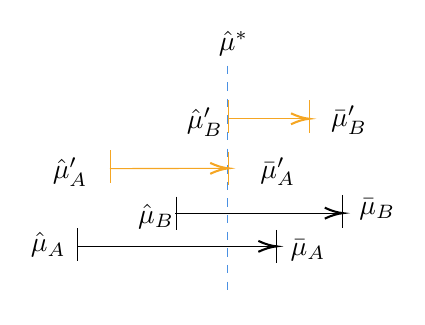
\begin{tikzpicture}[x=0.60pt,y=0.60pt,yscale=-1,xscale=1]
    \draw    (81.33,157.33) -- (199.33,157.33) ;
    \draw [shift={(201.33,157.33)}, rotate = 180] [color={rgb, 255:red, 0; green, 0; blue, 0 }  ][line width=0.75]    (10.93,-3.29) .. controls (6.95,-1.4) and (3.31,-0.3) .. (0,0) .. controls (3.31,0.3) and (6.95,1.4) .. (10.93,3.29)   ;
    \draw [dashed, color={rgb, 255:red, 74; green, 144; blue, 226 }  ,draw opacity=1 ]   (172,48.5) -- (172,187.5) ;
    \draw    (201.33,147.33) -- (201.33,167.33) ;
    \draw    (140.33,137.33) -- (239.33,137.33) ;
    \draw [shift={(241.33,137.33)}, rotate = 180] [color={rgb, 255:red, 0; green, 0; blue, 0 }  ][line width=0.75]    (10.93,-3.29) .. controls (6.95,-1.4) and (3.31,-0.3) .. (0,0) .. controls (3.31,0.3) and (6.95,1.4) .. (10.93,3.29)   ;
    \draw    (241.33,126.33) -- (241.33,146.33) ;
    \draw    (81.33,146.33) -- (81.33,166.33) ;
    \draw    (141.33,127.33) -- (141.33,147.33) ;
    \draw [color={rgb, 255:red, 245; green, 166; blue, 35 }  ,draw opacity=1 ]   (101,110.5) -- (170.33,110.34) ;
    \draw [shift={(172.33,110.33)}, rotate = 179.87] [color={rgb, 255:red, 245; green, 166; blue, 35 }  ,draw opacity=1 ][line width=0.75]    (10.93,-3.29) .. controls (6.95,-1.4) and (3.31,-0.3) .. (0,0) .. controls (3.31,0.3) and (6.95,1.4) .. (10.93,3.29)   ;
    \draw [color={rgb, 255:red, 245; green, 166; blue, 35 }  ,draw opacity=1 ]   (172.33,100.33) -- (172.33,120.33) ;
    \draw [color={rgb, 255:red, 245; green, 166; blue, 35 }  ,draw opacity=1 ]   (101.33,99.33) -- (101.33,119.33) ;
    \draw [color={rgb, 255:red, 245; green, 166; blue, 35 }  ,draw opacity=1 ]   (172,80.5) -- (219,80.5) ;
    \draw [shift={(221,80.5)}, rotate = 180] [color={rgb, 255:red, 245; green, 166; blue, 35 }  ,draw opacity=1 ][line width=0.75]    (10.93,-3.29) .. controls (6.95,-1.4) and (3.31,-0.3) .. (0,0) .. controls (3.31,0.3) and (6.95,1.4) .. (10.93,3.29)   ;
    \draw [color={rgb, 255:red, 245; green, 166; blue, 35 }  ,draw opacity=1 ]   (172.33,69.33) -- (172.33,89.33) ;
    \draw [color={rgb, 255:red, 245; green, 166; blue, 35 }  ,draw opacity=1 ]   (221.33,69.33) -- (221.33,89.33) ;

    % Text Node
    \draw (208.25,151.58) node [anchor=north west][inner sep=0.75pt]   [align=left] {$\bar{\mu}_A$};
    % Text Node
    \draw (51.8,147.51) node [anchor=north west][inner sep=0.75pt]   [align=left] {$\hat{\mu}_A$};
    % Text Node
    \draw (116.44,130.43) node [anchor=north west][inner sep=0.75pt]   [align=left] {$\hat{\mu}_B$};
    % Text Node
    \draw (249.69,127.16) node [anchor=north west][inner sep=0.75pt]   [align=left] {$\bar{\mu}_B$};
    % Text Node
    \draw (165,25.96) node [anchor=north west][inner sep=0.75pt]   [align=left] {$\hat{\mu}^*$};
    % Text Node
    \draw (65,102.51) node [anchor=north west][inner sep=0.75pt]   [align=left] {$\hat{\mu}_A'$};
    % Text Node
    \draw (145.8,72.51) node [anchor=north west][inner sep=0.75pt]   [align=left] {$\hat{\mu}_B'$};
    % Text Node
    \draw (190,102.16) node [anchor=north west][inner sep=0.75pt]   [align=left] {$\bar{\mu}_A'$};
    % Text Node
    \draw (232.69,71.16) node [anchor=north west][inner sep=0.75pt]   [align=left] {$\bar{\mu}_B'$};
\end{tikzpicture}

\end{document}